% Options for packages loaded elsewhere
\PassOptionsToPackage{unicode}{hyperref}
\PassOptionsToPackage{hyphens}{url}
\PassOptionsToPackage{dvipsnames,svgnames,x11names}{xcolor}
%
\documentclass[
  letterpaper,
  DIV=11,
  numbers=noendperiod]{scrartcl}

\usepackage{amsmath,amssymb}
\usepackage{iftex}
\ifPDFTeX
  \usepackage[T1]{fontenc}
  \usepackage[utf8]{inputenc}
  \usepackage{textcomp} % provide euro and other symbols
\else % if luatex or xetex
  \usepackage{unicode-math}
  \defaultfontfeatures{Scale=MatchLowercase}
  \defaultfontfeatures[\rmfamily]{Ligatures=TeX,Scale=1}
\fi
\usepackage{lmodern}
\ifPDFTeX\else  
    % xetex/luatex font selection
  \setmainfont[]{Times New Roman}
\fi
% Use upquote if available, for straight quotes in verbatim environments
\IfFileExists{upquote.sty}{\usepackage{upquote}}{}
\IfFileExists{microtype.sty}{% use microtype if available
  \usepackage[]{microtype}
  \UseMicrotypeSet[protrusion]{basicmath} % disable protrusion for tt fonts
}{}
\makeatletter
\@ifundefined{KOMAClassName}{% if non-KOMA class
  \IfFileExists{parskip.sty}{%
    \usepackage{parskip}
  }{% else
    \setlength{\parindent}{0pt}
    \setlength{\parskip}{6pt plus 2pt minus 1pt}}
}{% if KOMA class
  \KOMAoptions{parskip=half}}
\makeatother
\usepackage{xcolor}
\setlength{\emergencystretch}{3em} % prevent overfull lines
\setcounter{secnumdepth}{-\maxdimen} % remove section numbering
% Make \paragraph and \subparagraph free-standing
\ifx\paragraph\undefined\else
  \let\oldparagraph\paragraph
  \renewcommand{\paragraph}[1]{\oldparagraph{#1}\mbox{}}
\fi
\ifx\subparagraph\undefined\else
  \let\oldsubparagraph\subparagraph
  \renewcommand{\subparagraph}[1]{\oldsubparagraph{#1}\mbox{}}
\fi


\providecommand{\tightlist}{%
  \setlength{\itemsep}{0pt}\setlength{\parskip}{0pt}}\usepackage{longtable,booktabs,array}
\usepackage{calc} % for calculating minipage widths
% Correct order of tables after \paragraph or \subparagraph
\usepackage{etoolbox}
\makeatletter
\patchcmd\longtable{\par}{\if@noskipsec\mbox{}\fi\par}{}{}
\makeatother
% Allow footnotes in longtable head/foot
\IfFileExists{footnotehyper.sty}{\usepackage{footnotehyper}}{\usepackage{footnote}}
\makesavenoteenv{longtable}
\usepackage{graphicx}
\makeatletter
\def\maxwidth{\ifdim\Gin@nat@width>\linewidth\linewidth\else\Gin@nat@width\fi}
\def\maxheight{\ifdim\Gin@nat@height>\textheight\textheight\else\Gin@nat@height\fi}
\makeatother
% Scale images if necessary, so that they will not overflow the page
% margins by default, and it is still possible to overwrite the defaults
% using explicit options in \includegraphics[width, height, ...]{}
\setkeys{Gin}{width=\maxwidth,height=\maxheight,keepaspectratio}
% Set default figure placement to htbp
\makeatletter
\def\fps@figure{htbp}
\makeatother
% definitions for citeproc citations
\NewDocumentCommand\citeproctext{}{}
\NewDocumentCommand\citeproc{mm}{%
  \begingroup\def\citeproctext{#2}\cite{#1}\endgroup}
\makeatletter
 % allow citations to break across lines
 \let\@cite@ofmt\@firstofone
 % avoid brackets around text for \cite:
 \def\@biblabel#1{}
 \def\@cite#1#2{{#1\if@tempswa , #2\fi}}
\makeatother
\newlength{\cslhangindent}
\setlength{\cslhangindent}{1.5em}
\newlength{\csllabelwidth}
\setlength{\csllabelwidth}{3em}
\newenvironment{CSLReferences}[2] % #1 hanging-indent, #2 entry-spacing
 {\begin{list}{}{%
  \setlength{\itemindent}{0pt}
  \setlength{\leftmargin}{0pt}
  \setlength{\parsep}{0pt}
  % turn on hanging indent if param 1 is 1
  \ifodd #1
   \setlength{\leftmargin}{\cslhangindent}
   \setlength{\itemindent}{-1\cslhangindent}
  \fi
  % set entry spacing
  \setlength{\itemsep}{#2\baselineskip}}}
 {\end{list}}
\usepackage{calc}
\newcommand{\CSLBlock}[1]{\hfill\break\parbox[t]{\linewidth}{\strut\ignorespaces#1\strut}}
\newcommand{\CSLLeftMargin}[1]{\parbox[t]{\csllabelwidth}{\strut#1\strut}}
\newcommand{\CSLRightInline}[1]{\parbox[t]{\linewidth - \csllabelwidth}{\strut#1\strut}}
\newcommand{\CSLIndent}[1]{\hspace{\cslhangindent}#1}

\usepackage{hyperref}

% customize figure references
\renewcommand{\figureautorefname}{Fig.}

% toggle line numbers
\usepackage{lineno}
% \linenumbers

% toggle spacing
\usepackage{setspace}
\singlespacing
% \doublespacing

% make better hyphen for numeric ranges, \numrange{}{}
\usepackage[detect-none]{siunitx}
\sisetup{range-phrase = \text{--}}

% packages for mathematical notation
\usepackage{commath}
\KOMAoption{captions}{tableheading}
\addtokomafont{disposition}{\rmfamily}
\RedeclareSectionCommand[
  font=\normalfont\Large]{section}
\RedeclareSectionCommand[
  font=\normalfont\normalsize\bfseries]{subsection}
\RedeclareSectionCommand[
  font=\normalfont\normalsize\itshape]{subsubsection}
\RedeclareSectionCommand[
  font=\normalfont\normalsize,
  beforeskip=0.5\baselineskip, % space before the heading
  afterskip=0.5\baselineskip   % space after the heading (adjust this for spacing between heading and text)
]{paragraph}
\makeatletter
\@ifpackageloaded{caption}{}{\usepackage{caption}}
\AtBeginDocument{%
\ifdefined\contentsname
  \renewcommand*\contentsname{Table of contents}
\else
  \newcommand\contentsname{Table of contents}
\fi
\ifdefined\listfigurename
  \renewcommand*\listfigurename{List of Figures}
\else
  \newcommand\listfigurename{List of Figures}
\fi
\ifdefined\listtablename
  \renewcommand*\listtablename{List of Tables}
\else
  \newcommand\listtablename{List of Tables}
\fi
\ifdefined\figurename
  \renewcommand*\figurename{Figure}
\else
  \newcommand\figurename{Figure}
\fi
\ifdefined\tablename
  \renewcommand*\tablename{Table}
\else
  \newcommand\tablename{Table}
\fi
}
\@ifpackageloaded{float}{}{\usepackage{float}}
\floatstyle{ruled}
\@ifundefined{c@chapter}{\newfloat{codelisting}{h}{lop}}{\newfloat{codelisting}{h}{lop}[chapter]}
\floatname{codelisting}{Listing}
\newcommand*\listoflistings{\listof{codelisting}{List of Listings}}
\makeatother
\makeatletter
\makeatother
\makeatletter
\@ifpackageloaded{caption}{}{\usepackage{caption}}
\@ifpackageloaded{subcaption}{}{\usepackage{subcaption}}
\makeatother
\ifLuaTeX
  \usepackage{selnolig}  % disable illegal ligatures
\fi
\usepackage{bookmark}

\IfFileExists{xurl.sty}{\usepackage{xurl}}{} % add URL line breaks if available
\urlstyle{same} % disable monospaced font for URLs
\hypersetup{
  pdftitle={Is photosynthetic capacity associated with diversification of C\_3 plants?},
  colorlinks=true,
  linkcolor={blue},
  filecolor={Maroon},
  citecolor={Blue},
  urlcolor={Blue},
  pdfcreator={LaTeX via pandoc}}

\title{Is photosynthetic capacity associated with diversification of
C\(_3\) plants?}
\author{}
\date{}

\begin{document}
\maketitle

\begin{center}
Christopher D. Muir$^{1,*}$
\end{center}

\(^1\) Department of Botany, University of Wisconsin, Madison, WI, USA
53706

\(^*\) Corresponding author: Christopher D. Muir, cdmuir@wisc.edu

Author contributions: CDM conceived of the ideas and wrote the
manuscript.

Data availability statement: Data are available from previously
published sources. The code to reproduce analyses is available on GitHub
(https://github.com/cdmuir/photosynthesis-diversification) and archived
on Zenodo.

Word count: 63 in Abstract; 1,038 in Main text

Running head: Photosynthetic capacity and diversification

Keywords: ancestral state reconstruction, diversification,
macroevolution, photosynthesis, phylogenetic comparative methods

\newpage

\subsection{Abstract}\label{abstract}

Schweiger \& Schweiger (2024) recently proposed that evolution of
greater photosynthetic capacity in C\(_3\) plant species may be linked
to increased species diversification. This conclusion is premature
because their methods cannot reliably estimate diversification rate or
ancestral trait values. Reanalyzing the data set using model-based
phylogenetic comparative methods reveals no evidence that photosynthetic
capacity is associated with diversification rates among C\(_3\) plant
genera.

\subsection{Main text}\label{main-text}

Phylogenetic comparative methods (PCMs) are widely used to infer
historical patterns of species diversification and phenotypic evolution
based on the relationships among extant species and their trait values
(Pennell \& Harmon 2013). Recently Schweiger \& Schweiger (2024) purport
to show that greater photosynthetic capacity is linked to greater
diversification among C\(_3\) vascular land plants over the past 80
million years. Specifically, they argue that diversification rates
increased along with photosynthetic capacity (\(V_\mathrm{cmax}\) and
\(J_\mathrm{max}\)) as atmospheric CO\(_2\) decreased throughout the
Miocene. This conclusion is premature because the PCMs Schweiger \&
Schweiger (2024) use to estimate diversification rates and ancestral
states do not account for and are highly sensitive to incomplete taxon
sampling.

\subsubsection{Diversification analysis}\label{diversification-analysis}

Diversification rates are typically inferred using the distribution of
branch lengths in a molecular phylogeny. The reconstructed evolutionary
process, even with complete sampling of extant taxa and perfect
information, cannot infer the presence of lineages that left no
descendants because of extinction (Nee \emph{et al.} 1994b). Incomplete
taxon sampling acts like a recent extinction event because nodes leading
to unsampled taxa cannot be inferred. Valid inference of diversification
rates must therefore condition on both extinction and incomplete
sampling. Schweiger \& Schweiger (2024) analyze a molecular phylogeny of
vascular land plants containing 232 species, 0.065\% of the 359,208
currently accepted species as of December 2024 (Kindt 2020). They
estimate diversification rate as \(\log \left(n\right) / t\), where
\(n\) is the number of tips and \(t\) is the stem group age (Magallon \&
Sanderson 2001). Since apparent \(n\) is a small fraction of its true
value, this statistic cannot estimate diversification rate. The
Kendall-Moran estimate of speciation rate used by Schweiger \& Schweiger
(2024) works for completely sampled phylogenies with no extinction
(Baldwin \& Sanderson 1998), an untenable assumption in this case.
Schweiger \& Schweiger (2024) compound these errors by pruning tips and
branches younger than each time interval for which they estimate
diversification rates. Thus, at each interval they artificially remove
nodes in the phylogeny, further biasing downward estimates of
diversification.

Random incomplete sampling biases downward estimates of diversification
rates in the recent past (Nee \emph{et al.} 1994a). The bias caused by
random incomplete sampling is opposite the pattern Schweiger \&
Schweiger (2024) observe of more rapid diversification toward the
present. Apparent increases in diversification in younger clades is a
general phenomenon not confined to C\(_3\) plants (Harmon \emph{et al.}
2021) that may be a result of bias toward sampling species-rich clades
(Louca \emph{et al.} 2022). Reliable inference must address both
incomplete and nonrandom sampling.

\subsubsection{Ancestral trait analysis}\label{ancestral-trait-analysis}

Unobserved ancestral states must be reconstructed using a probabilistic
model of trait evolution, but inferred states are often impossible to
independently verify (but see Polly 2001). There is a high likelihood
that estimates from misspecified models are misleading (Revell 2025).
Schweiger \& Schweiger (2024) do not estimate ancestral states based on
a trait model, but instead calculate it as the ``median trait values
from all species that originated in the respective time period,'' where
time period refers to a 5-million-year interval. There are two
fundamental errors with this approach. First, because the phylogeny
contains a small fraction of all species, the origin time of a species
(when it split from its sister species) will be biased upward by an
unpredictable amount (Figure~\ref{fig-phy1}a). The nodes used by
Schweiger \& Schweiger (2024) are on average 315\% older than and
modestly correlated with (log-log \(r^2 = 0.43\)) the nodes separating
nearest species in the unpruned Zanne \emph{et al.} (2014) tree, which
itself contains 31,389 species, representing only 8.7\% of described
vascular land plant species.

\begin{figure}

\centering{

\includegraphics{ms_files/figure-pdf/fig-phy1-1.pdf}

}

\caption{\label{fig-phy1}(Caption next page.)}

\end{figure}%

\addtocounter{figure}{-1}
\begin{figure}[t!]
\caption{(Previous page). The method Schweiger \& Schweiger (2024) use to infer when a species originated is misleading when taxon sampling is incomplete. (A) For example, the Hawaiian lobeliads \textit{Brighamia insignis} A. Gray and \textit{Delissea rhytidosperma} H. Mann in their data set are inferred by this method to have ``originated'' 5.23 mya, as shown in the phylogeny above. This apparent origin (black point on more ancient node) is an artifact of more closely related congeneric species (*B. rockii* H. St. John and *D. subcordata* Gaudich.) not being sampled (dashed branches leading to unsampled species). The node of the apparent origin represents the most recent common ancestor of these species, but both species actually diverged from more closely related species much more recently (white points). The timing of divergence from putative sister species is approximate and for illustration purposes only (based on Givnish \textit{et al.} 2009). (B) The consequences of this methodological choice are that the divergence times used by Schweiger \& Schweiger (2024) ($y$-axis) are biased upward by an average of 315\% and modestly correlated ($r^2 = 0.43$ on log-log scale) with the divergence times estimated from the full phylogeny ($x$-axis) from Zanne \textit{et al.} (2014). Those divergence times are themselves only loosely related to the true divergence time between sister species because of mostly incomplete sampling even in the unpruned Zanne \textit{et al.} (2014) phylogeny.}
\end{figure}

Second, the method for estimating average trait values in past intervals
implies strong and unrealistic assumptions about trait evolution, is
inappropriate for a sparsely sampled phylogeny, and is highly sensitive
to small differences in taxon sampling. Even if species' origination
dates were inferred correctly, estimating ancestral states by assuming
they are equal to the state of the extant descendant implies all trait
evolution occurs during speciation events (cladogenic) and not along
lineages (anagenic). Assuming cladogenic evolution is especially
problematic in this case because most nodes in the phylogeny are not
sampled, thereby missing most cladogenic events when trait change would
occur by their implied assumptions. A median of 7 nodes per species were
pruned from the Zanne \emph{et al.} (2014) phylogeny in their analysis,
but this is a severe undercount of missing nodes because of both
incomplete sampling in the unpruned tree and extinction. Finally,
estimates of past trait values using this method are highly sensitive to
small changes in taxon sampling. A minor change in sampling can result
in quite different estimates even with the same underlying evolutionary
scenario (see Figure~\ref{fig-phy2} for a worked example).

\begin{figure}

\centering{

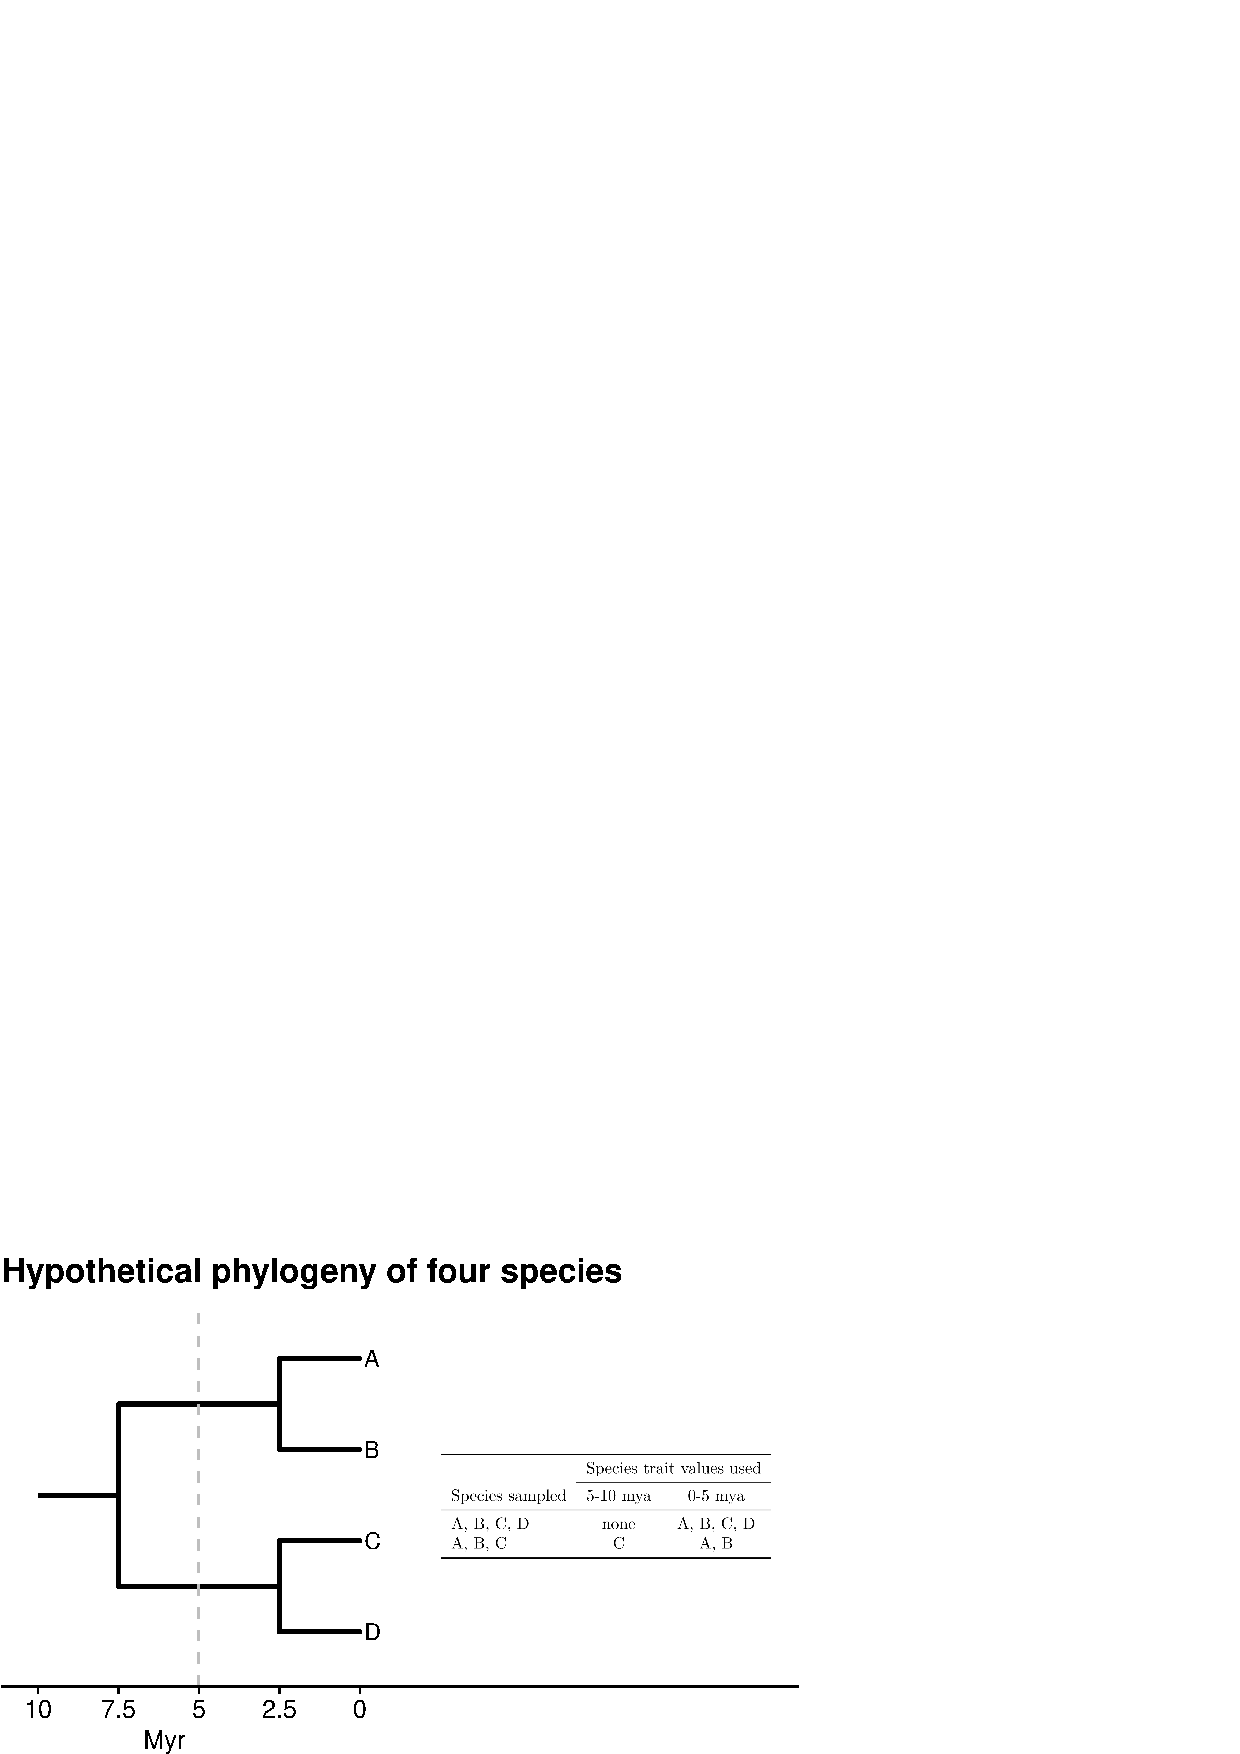
\includegraphics{ms_files/figure-pdf/fig-phy2-1.pdf}

}

\caption{\label{fig-phy2}The method Schweiger \& Schweiger (2024) use to
estimate ancestral trait values is sensitive to small differences in
taxon sampling. Assume we know the true phylogeny of four species A, B,
C, and D (left). The species A and B are sister species that split 2.5
mya, likewise for C and D. The common ancestor of all four split 7.5
mya. If we sampled all four species, their trait values would contribute
to the estimated average trait value in the interval between 0 and 5
mya. This clade would not contribute to the estimated average trait
value in the interval between 5 and 10 mya because the species did not
originate in that interval. However, it is clear that the ancestors of
these species must have existed during that interval. Now consider the
effect of incomplete sampling. If species D were not sampled, then the
trait values for A and B would contribute to the 0-5 mya interval and
species C would contribute to the 5-10 mya interval.The species used to
calculate average trait values at different time intervals changes
depending on whether all species are sampled or a subset are sampled
(right), even though the underlying biological reality is unchanged.}

\end{figure}%

\subsubsection{No evidence that photosynthetic capacity is linked to
diversification in seed
plants}\label{no-evidence-that-photosynthetic-capacity-is-linked-to-diversification-in-seed-plants}

Several PCMs have been developed in the past decade to estimate whether
diversification rates vary among lineages and through time in
association with traits (Martínez-Gómez \emph{et al.} 2024; Morlon
\emph{et al.} 2024). These methods account for extinction and incomplete
sampling and therefore can, in principle, test whether diversification
is associated with traits like \(V_\text{cmax}\) or \(J_\text{max}\).
When extinction and incomplete sampling are accounted for using BAMM
version 2.5.0 (Rabosky 2014) on a nearly-complete phylogeny of seed
plant genera (Dimitrov \emph{et al.} 2023), there is no evidence that
speciation or net diversification rates are associated with
\(V_\text{cmax}\) or \(J_\text{max}\) (Figure~\ref{fig-strapp}) based on
permutation tests developed by Rabosky \& Huang (2016) (see Supporting
Information). This method answers a slightly different question than
that posed by Schweiger \& Schweiger (2024) because it tests for an
association between tip rates and traits, not ancestral rates and
traits. However, the tip rates of many genera encompass much of the
Miocene when global CO\(_2\) declined and tip rates suffer from fewer
identifiability issues (Louca \& Pennell 2020). Alternative methods not
considered here are CLaDS2 (Barido-Sottani \& Morlon 2023) and QuaSSE
(FitzJohn 2010). While these PCMs account for extinction and incomplete
sampling, no method performs well when taxon sampling is extremely
sparse, samples are biased, or when making inferences about the deep
past from extant taxa. Certain questions may be better suited to
specific clades with (near-)complete sampling (Donoghue \& Edwards
2019), well resolved and fossil-calibrated nodes, and to relatively
recent geological epochs.

\begin{figure}

\centering{

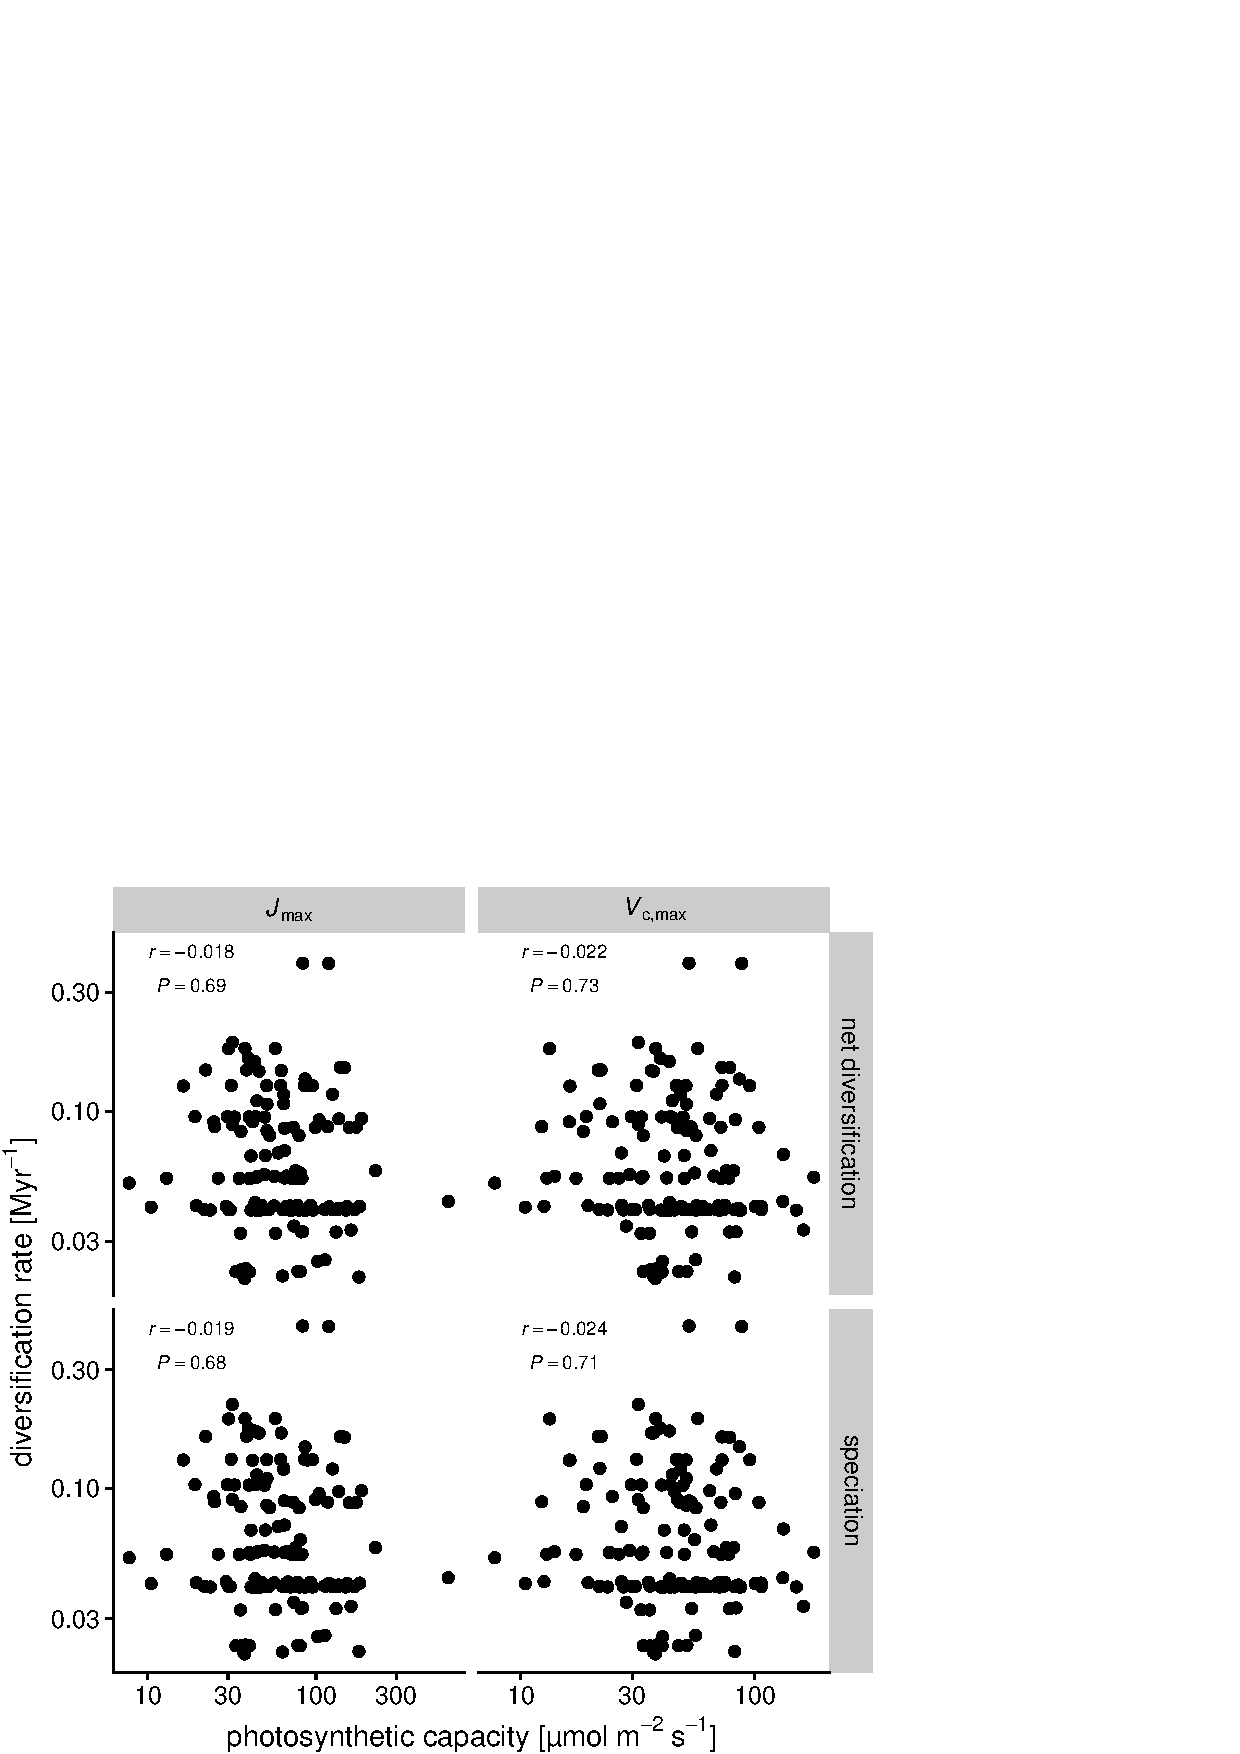
\includegraphics{ms_files/figure-pdf/fig-strapp-1.pdf}

}

\caption{\label{fig-strapp}No evidence that photosynthetic capacity
explains variation in speciation or net diversification rates among
C\(_3\) seed plant genera. Net diversification (top row) and speciation
(bottom row) rates estimated using BAMM version 2.5.0 on a
nearly-complete phylogeny of seed plant genera (Dimitrov \emph{et al.}
2023) are not significantly associated with average \(J_\mathrm{max}\)
(left column) or \(V_\mathrm{cmax}\) (right column) based on STRAPP
permutation tests (Rabosky \& Huang 2016). Both axes are log-scaled. The
estimated Pearson product moment correlation \(r\) and permutation based
\(P\)-values from two-tailed tests are in the upper-left of each facet.}

\end{figure}%

\subsection{Acknowledgments}\label{acknowledgments}

Andreas Schweiger and two anonymous reviewers provided constructive
feedback on an earlier draft of this manuscript. CDM is supported by the
National Science Foundation (DEB-2131817). Support for this research was
provided by the Office of the Vice Chancellor for Research and Graduate
Education at the University of Wisconsin-Madison with funding from the
Wisconsin Alumni Research Foundation. The author declares no conflicts
of interest.

\clearpage

\section{References}\label{references}

\phantomsection\label{refs}
\begin{CSLReferences}{1}{0}
\bibitem[\citeproctext]{ref-baldwin_age_1998}
Baldwin, B.G. \& Sanderson, M.J. (1998).
\href{https://doi.org/10.1073/pnas.95.16.9402}{Age and rate of
diversification of the {Hawaiian} silversword alliance ({Compositae})}.
\emph{Proceedings of the National Academy of Sciences}, 95, 9402--9406.

\bibitem[\citeproctext]{ref-barido-sottani_clads_2023}
Barido-Sottani, J. \& Morlon, H. (2023).
\href{https://doi.org/10.1093/sysbio/syad027}{The {ClaDS}
rate-heterogeneous birth--death prior for full phylogenetic inference in
{BEAST2}}. \emph{Systematic Biology}, 72, 1180--1187.

\bibitem[\citeproctext]{ref-dimitrov_diversification_2023}
Dimitrov, D., Xu, X., Su, X., Shrestha, N., Liu, Y., Kennedy, J.D.,
\emph{et al.} (2023).
\href{https://doi.org/10.1038/s41467-023-43396-8}{Diversification of
flowering plants in space and time}. \emph{Nature Communications}, 14,
7609.

\bibitem[\citeproctext]{ref-donoghue_model_2019}
Donoghue, M.J. \& Edwards, E.J. (2019).
\href{https://doi.org/10.1002/ajb2.1255}{Model clades are vital for
comparative biology, and ascertainment bias is not a problem in
practice: A response to {Beaulieu} and {O}'{Meara} (2018)}.
\emph{American Journal of Botany}, 106, 327--330.

\bibitem[\citeproctext]{ref-fitzjohn_quantitative_2010}
FitzJohn, R.G. (2010).
\href{https://doi.org/10.1093/sysbio/syq053}{Quantitative {Traits} and
{Diversification}}. \emph{Systematic Biology}, 59, 619--633.

\bibitem[\citeproctext]{ref-givnish_origin_2009}
Givnish, T.J., Millam, K.C., Mast, A.R., Paterson, T.B., Theim, T.J.,
Hipp, A.L., \emph{et al.} (2009).
\href{https://doi.org/10.1098/rspb.2008.1204}{Origin, adaptive radiation
and diversification of the {Hawaiian} lobeliads ({Asterales}:
{Campanulaceae})}. \emph{Proceedings of the Royal Society B: Biological
Sciences}, 276, 407--416.

\bibitem[\citeproctext]{ref-harmon_causes_2021}
Harmon, L.J., Pennell, M.W., Henao-Diaz, L.F., Rolland, J., Sipley, B.N.
\& Uyeda, J.C. (2021).
\href{https://doi.org/10.1146/annurev-ecolsys-011921-023644}{Causes and
{Consequences} of {Apparent} {Timescaling} {Across} {All} {Estimated}
{Evolutionary} {Rates}}. \emph{Annual Review of Ecology, Evolution, and
Systematics}, 52, 587--609.

\bibitem[\citeproctext]{ref-kindt_worldflora_2020}
Kindt, R. (2020).
\href{https://doi.org/10.1002/aps3.11388}{{WorldFlora}: {An} {R} package
for exact and fuzzy matching of plant names against the {World} {Flora}
{Online} taxonomic backbone data}. \emph{Applications in Plant
Sciences}, 8, e11388.

\bibitem[\citeproctext]{ref-louca_scaling_2022}
Louca, S., Henao-Diaz, L.F. \& Pennell, M. (2022).
\href{https://doi.org/10.1111/evo.14515}{The scaling of diversification
rates with age is likely explained by sampling bias}. \emph{Evolution},
76, 1625--1637.

\bibitem[\citeproctext]{ref-louca_extant_2020}
Louca, S. \& Pennell, M.W. (2020).
\href{https://doi.org/10.1038/s41586-020-2176-1}{Extant timetrees are
consistent with a myriad of diversification histories}. \emph{Nature},
580, 502--505.

\bibitem[\citeproctext]{ref-magallon_absolute_2001}
Magallon, S. \& Sanderson, M.J. (2001).
\href{https://doi.org/10.1111/j.0014-3820.2001.tb00826.x}{Absolute
diversification rates in angiosperm clades}. \emph{Evolution}, 55,
1762--1780.

\bibitem[\citeproctext]{ref-martinez-gomez_commonly_2024}
Martínez-Gómez, J., Song, M.J., Tribble, C.M., Kopperud, B.T., Freyman,
W.A., Höhna, S., \emph{et al.} (2024).
\href{https://doi.org/10.1093/evlett/qrad044}{Commonly used {Bayesian}
diversification methods lead to biologically meaningful differences in
branch-specific rates on empirical phylogenies}. \emph{Evolution
Letters}, 8, 189--199.

\bibitem[\citeproctext]{ref-morlon_phylogenetic_2024}
Morlon, H., Andréoletti, J., Barido-Sottani, J., Lambert, S.,
Perez-Lamarque, B., Quintero, I., \emph{et al.} (2024).
\href{https://doi.org/10.1146/annurev-ecolsys-102722-020508}{Phylogenetic
{Insights} into {Diversification}}. \emph{Annual Review of Ecology,
Evolution, and Systematics}, 55, 1--21.

\bibitem[\citeproctext]{ref-nee_extinction_1994}
Nee, S., Holmes, E.C., May, R.M. \& Harvey, P.H. (1994a).
\href{https://doi.org/10.1098/rstb.1994.0054}{Extinction rates can be
estimated from molecular phylogenies}. \emph{Philosophical Transactions
of the Royal Society of London. Series B: Biological Sciences}, 344,
77--82.

\bibitem[\citeproctext]{ref-nee_reconstructed_1994}
Nee, S., May, R.M. \& Harvey, P.H. (1994b).
\href{http://www.jstor.org/stable/55922}{The {Reconstructed}
{Evolutionary} {Process}}. \emph{Philosophical Transactions: Biological
Sciences}, 344, 305--311.

\bibitem[\citeproctext]{ref-pennell_integrative_2013}
Pennell, M.W. \& Harmon, L.J. (2013).
\href{https://doi.org/10.1111/nyas.12157}{An integrative view of
phylogenetic comparative methods: Connections to population genetics,
community ecology, and paleobiology}. \emph{Annals of the New York
Academy of Sciences}, 1289, 90--105.

\bibitem[\citeproctext]{ref-polly_paleontology_2001}
Polly, P.D. (2001). \href{https://doi.org/10.1086/320622}{Paleontology
and the {Comparative} {Method}: {Ancestral} {Node} {Reconstructions}
versus {Observed} {Node} {Values}}. \emph{The American Naturalist}, 157,
596--609.

\bibitem[\citeproctext]{ref-rabosky_automatic_2014}
Rabosky, D.L. (2014).
\href{https://doi.org/10.1371/journal.pone.0089543}{Automatic
{Detection} of {Key} {Innovations}, {Rate} {Shifts}, and
{Diversity}-{Dependence} on {Phylogenetic} {Trees}}. \emph{PLoS ONE}, 9,
e89543.

\bibitem[\citeproctext]{ref-rabosky_robust_2016}
Rabosky, D.L. \& Huang, H. (2016).
\href{https://doi.org/10.1093/sysbio/syv066}{A {Robust}
{Semi}-{Parametric} {Test} for {Detecting} {Trait}-{Dependent}
{Diversification}}. \emph{Systematic Biology}, 65, 181--193.

\bibitem[\citeproctext]{ref-revell_ancestral_2025}
Revell, L.J. (2025).
\href{https://doi.org/10.1007/s11692-025-09645-y}{Ancestral {State}
{Reconstruction} of {Phenotypic} {Characters}}. \emph{Evolutionary
Biology}, 52, 1--25.

\bibitem[\citeproctext]{ref-schweiger_significant_2024}
Schweiger, A.H. \& Schweiger, J.M.-I. (2024).
\href{https://doi.org/10.1111/ele.14523}{Significant {Links} {Between}
{Photosynthetic} {Capacity}, {Atmospheric} {CO}\(_{\textrm{2}}\) and the
{Diversification} of {C}\(_{\textrm{3}}\) {Plants} {During} the {Last}
80 {Million} {Years}}. \emph{Ecology Letters}, 27, e14523.

\bibitem[\citeproctext]{ref-zanne_three_2014}
Zanne, A.E., Tank, D.C., Cornwell, W.K., Eastman, J.M., Smith, S.A.,
FitzJohn, R.G., \emph{et al.} (2014).
\href{https://doi.org/10.1038/nature12872}{Three keys to the radiation
of angiosperms into freezing environments}. \emph{Nature}, 506, 89--92.

\end{CSLReferences}

\clearpage

\section{Supporting Information}\label{supporting-information}

\subsection{Estimating the relationshp between photosynthetic capacity
and diversification rates using
BAMM}\label{estimating-the-relationshp-between-photosynthetic-capacity-and-diversification-rates-using-bamm}

The speciation and net diversification rates estimated by Dimitrov
\emph{et al.} (2023) were unavailable from the authors, but I reanalyzed
their molecular phylogeny of seed plant genera using their sampling
fractions and following the same procedures in BAMM as described in
their paper. For the STRAPP analysis, I estimated the correlation
between log-transformed rates and traits using 1000 permutations to
generate the null distribution of the Pearson product-moment
correlation. The \(V_\mathrm{c,max}\) and \(J_\mathrm{max}\) trait data
from Schweiger \& Schweiger (2024) were averaged at the genus level when
more than one species per genus was present. This was necessary because
Dimitrov \emph{et al.} (2023) estimated a single diversification rate
per genus. Although this method uses macroevolutionary models to account
for extinction and incomplete sampling, the results should be
interpreted with extreme caution. For example, it does not account for
uncertainty in the phylogeny, the species sampling is extremely sparse,
variation within genera is ignored, and temporal variation in
diversification rates may not be identifiable from extant taxa only
(Louca \& Pennell 2020).



\end{document}
